\documentclass[12pt,letterpaper]{article}
\usepackage[margin=.63in,headheight=15pt,headsep=19pt,footskip=25pt]{geometry}
\usepackage{tikz,fancyhdr}
\usetikzlibrary{arrows.meta,patterns}
\renewcommand{\familydefault}{\sfdefault}
\pagestyle{fancy}\fancyhf{}\renewcommand{\headrulewidth}{.4pt}
\fancyhead[L]{\small Week 22 / Meeting regions encore / Grades 2--5}
\fancyfoot[L]{\small Bellingham Math Circle / Week 22 / W22-BON-v1}\fancyfoot[R]{\small\thepage}
\setlength{\parindent}{0pt}\setlength{\parskip}{8pt}
\newcommand{\problem}[2]{\textbf{Problem #1:} #2\par}
\newcommand{\lines}[1]{\foreach \i in {1,...,#1}{\par\vspace{10pt}\hrulefill}\par}
\newcommand{\genericdots}{\foreach \x/\y/\lab in {1/0/A,5/0/B,8/2/C,7/6/D,3/7/E,0/3/F}{\fill (\x,\y) circle (2pt);\node[font=\small,above right] at (\x,\y){\lab};}}
\begin{document}
A group's region is the filled shape inside a stretched band around its dots, including its edge. One dot gives a point; two dots give a segment. Dot centers define the points.

\begin{center}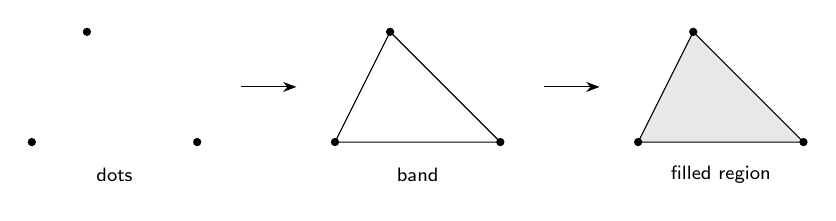
\begin{tikzpicture}[x=7mm,y=7mm]
\foreach \x/\y in {0/0,3/0,1/2}{\fill (\x,\y) circle (1.5pt);}
\draw[-{Stealth}] (3.8,1)--(4.8,1);
\draw (5.5,0)--(8.5,0)--(6.5,2)--cycle;\foreach \x/\y in {5.5/0,8.5/0,6.5/2}{\fill (\x,\y) circle (1.5pt);}
\draw[-{Stealth}] (9.3,1)--(10.3,1);
\filldraw[fill=gray!18] (11,0)--(14,0)--(12,2)--cycle;\foreach \x/\y in {11/0,14/0,12/2}{\fill (\x,\y) circle (1.5pt);}
\node[font=\scriptsize] at (1.5,-.6){dots};\node[font=\scriptsize] at (7,-.6){band};\node[font=\scriptsize] at (12.5,-.6){filled region};
\end{tikzpicture}\end{center}

\problem{1}{Keep as few of these dots as possible while keeping T in their region. Mark the dots you keep and draw their region.}
\begin{center}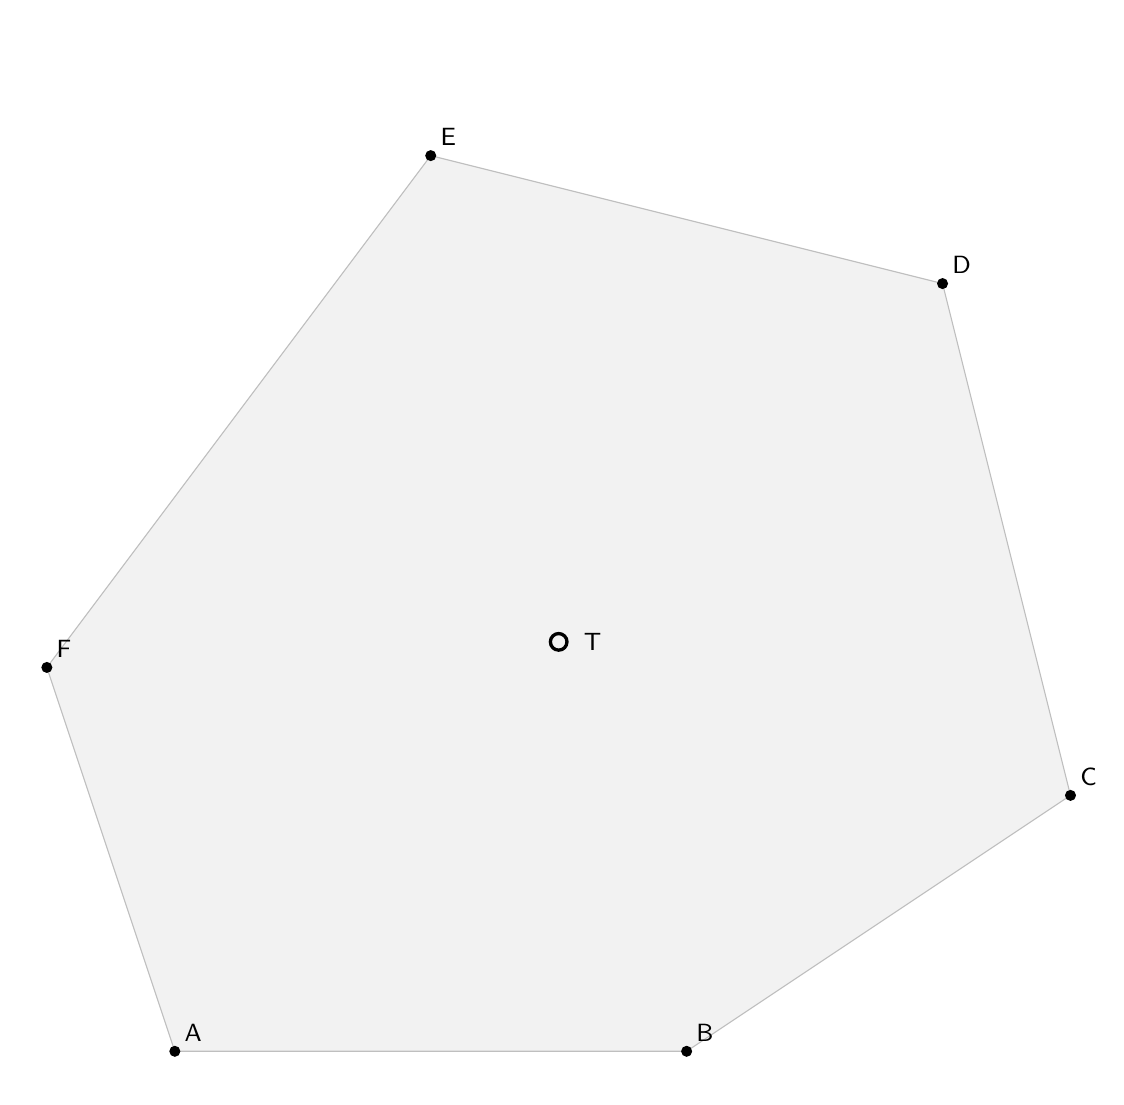
\begin{tikzpicture}[x=16.25mm,y=16.25mm]
\useasboundingbox (-.15,-.2) rectangle (8.2,8);
\filldraw[fill=gray!10,draw=gray!50] (1,0)--(5,0)--(8,2)--(7,6)--(3,7)--(0,3)--cycle;
\genericdots\draw[very thick] (4,3.2) circle (3pt);\node[font=\small,right] at (4.12,3.2){T};
\end{tikzpicture}\end{center}
\problem{2}{On a tracing copy, place targets that need exactly one, exactly two, and exactly three kept dots. Could a target inside the original region ever need four? Explain.}
\lines{2}
\newpage
\problem{3}{For each grouping below, find a straight line with one whole group strictly on each side and no dot on the line. If a grouping has no such line, show why. Use tracing copies to keep the two attempts separate.}
\begin{center}\begin{tabular}{c@{\qquad}c}
first grouping&second grouping\\[4pt]
AC / BD&AB / CD
\end{tabular}\end{center}
\begin{center}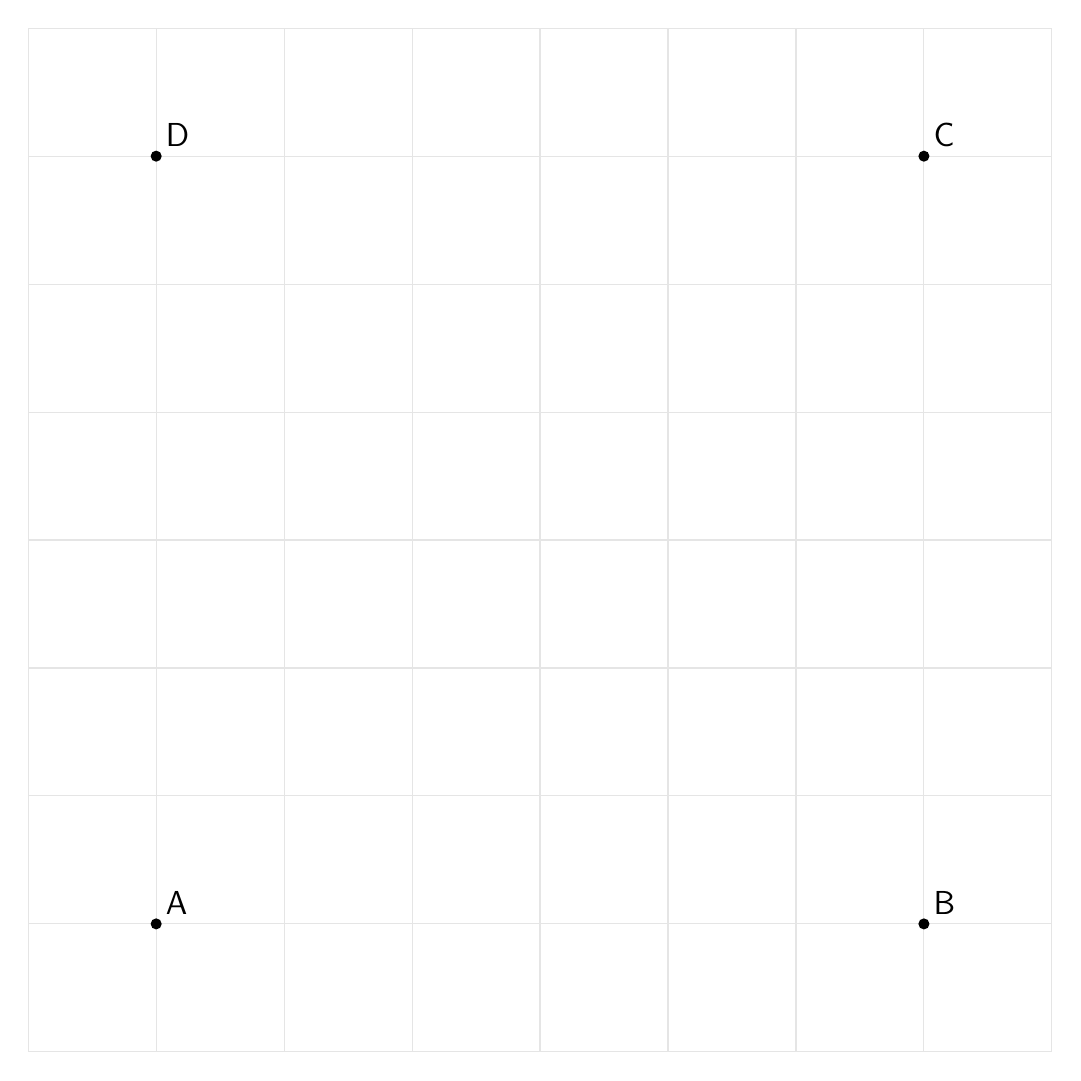
\begin{tikzpicture}[x=16.25mm,y=16.25mm]
\draw[gray!20,step=1] (0,0) grid (8,8);
\foreach \x/\y/\lab in {1/1/A,7/1/B,7/7/C,1/7/D}{\fill (\x,\y) circle (2pt);\node[font=\large,above right] at (\x,\y){\lab};}
\end{tikzpicture}\end{center}
\lines{5}
\newpage
\problem{4}{Use each row separately. Split every label into three nonempty groups so their three regions share one point. Mark that common point. For any impossible row, explain why no split works.}
\begin{center}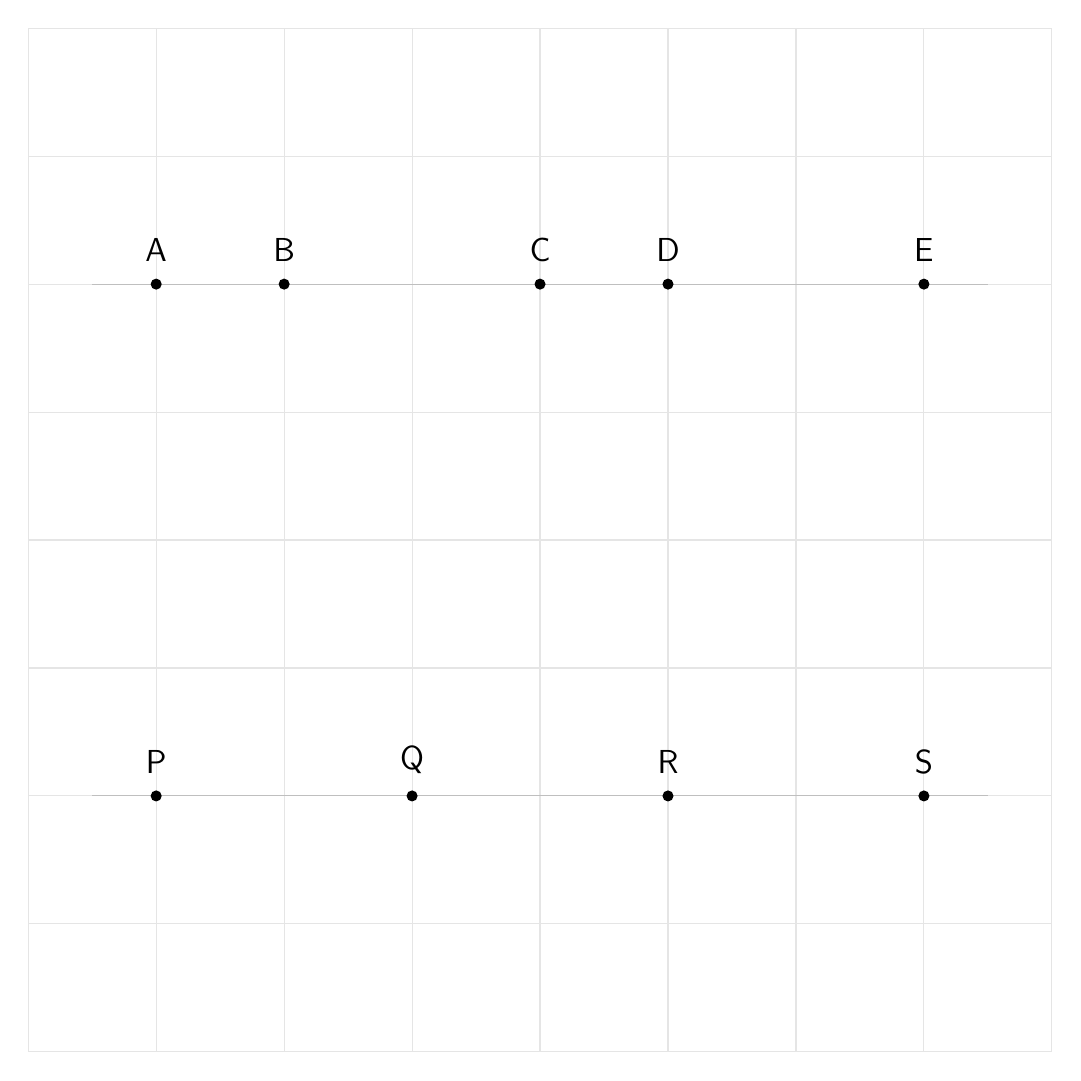
\begin{tikzpicture}[x=16.25mm,y=16.25mm]
\draw[gray!20,step=1] (0,0) grid (8,8);
\draw[gray!50] (.5,6)--(7.5,6) (.5,2)--(7.5,2);
\foreach \x/\lab in {1/A,2/B,4/C,5/D,7/E}{\fill (\x,6) circle (2pt);\node[font=\large,above] at (\x,6.1){\lab};}
\foreach \x/\lab in {1/P,3/Q,5/R,7/S}{\fill (\x,2) circle (2pt);\node[font=\large,above] at (\x,2.1){\lab};}
\end{tikzpicture}\end{center}
\lines{5}
\newpage
\problem{5}{Split all six labels into three nonempty groups so their three regions share one point. Draw the regions and mark one point in all three.}
\begin{center}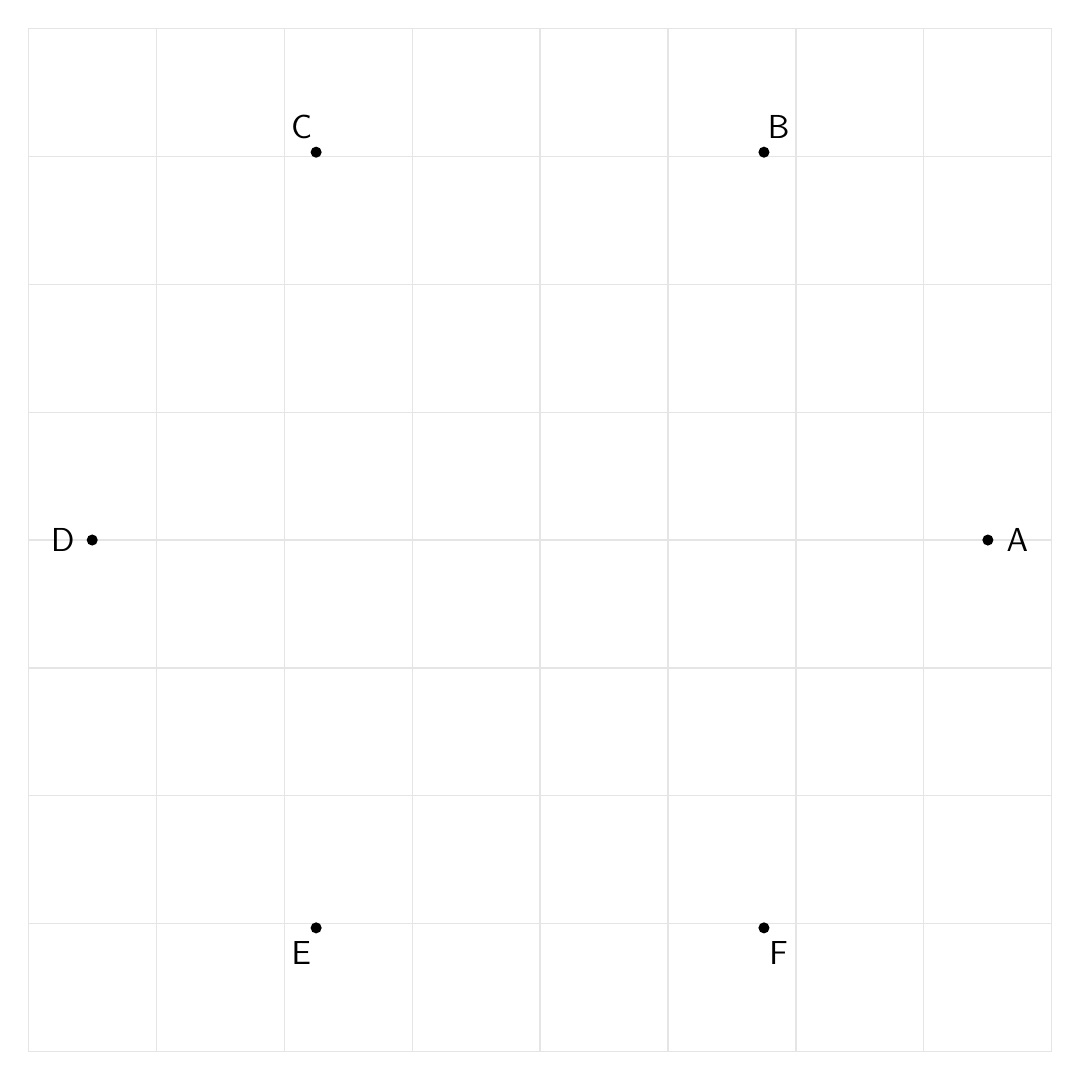
\begin{tikzpicture}[x=16.25mm,y=16.25mm]
\draw[gray!20,step=1] (0,0) grid (8,8);
\foreach \a/\lab in {0/A,60/B,120/C,180/D,240/E,300/F}{\coordinate (\lab) at ({4+3.5*cos(\a)},{4+3.5*sin(\a)});\fill (\lab) circle (2pt);\node[font=\large,shift={({.23*cos(\a)},{.23*sin(\a)})}] at (\lab){\lab};}
\end{tikzpicture}\end{center}
\lines{5}
\newpage
\problem{6}{Can these six labels be split into three nonempty groups whose regions share one point? Draw a successful split, or explain why every split fails. Meeting at three different points does not count.}
\begin{center}\begin{tikzpicture}[x=16.25mm,y=16.25mm]
\useasboundingbox (-.15,-.2) rectangle (8.2,8);
\draw[gray!20,step=1] (0,0) grid (8,8);\genericdots
\end{tikzpicture}\end{center}
\lines{5}
\end{document}
